%%%%Select the class of document
\documentclass{amsart} %type/class of article
%\documentclass{article}
%\documentclass{book}
%\documentclass{letter}

%%%%Select packages
\usepackage{amsthm,amsmath,amssymb} %math packages (always include)
\usepackage{geometry} %can be used to modify page dimensions, etc.
\usepackage{graphicx} %figure
\usepackage{float} %figure position in pdf
\usepackage{multirow} %table with multirow
\usepackage[labelfont=rm]{subcaption} %subcaption of figure
\usepackage[numbers]{natbib} %management of bibliography
\usepackage{listings} %use to list command or else in block
\usepackage{xcolor}  %allow to display color
\usepackage{url}
\usepackage{placeins}
\usepackage{algorithm}
\usepackage[noend]{algpseudocode}
%%%%% End Select packages


%%%% Define a style used to display a block of Latex code
\lstdefinestyle{TexStyle}{
language={[LaTeX]TeX},
frame=single,
backgroundcolor=\color{white},
basicstyle=\small\ttfamily,
morekeywords={maketitle,includegraphics},
keywordstyle=\color{blue},  
commentstyle=\color{gray},
stringstyle=\color{black}
}
\definecolor{dkgreen}{rgb}{0,0.6,0}
\definecolor{gray}{rgb}{0.5,0.5,0.5}
\definecolor{mauve}{rgb}{0.58,0,0.82}

\lstset{frame=tb,
	language=C,
	aboveskip=3mm,
	belowskip=3mm,
	showstringspaces=false,
	columns=flexible,
	basicstyle={\small\ttfamily},
	numbers=none,
	numberstyle=\tiny\color{gray},
	keywordstyle=\color{blue},
	commentstyle=\color{dkgreen},
	stringstyle=\color{mauve},
	breaklines=true,
	breakatwhitespace=true,
	tabsize=2
}    


%%%% Set up title page information
\title{CAAM 520: Computational Science II \\
Homework 3.}
\author{Wei Wu}
%\date{\today}
%%%% End Set up title page information


%%% Begin document
\begin{document}

%%%% Write an abstract if needed
%\begin{abstract}
%You can add an abstract at the beginning of the article.
%\end{abstract}

%%%% Make title page
\maketitle

\section{Introduction} 

In this project, we build upon the previous project: we parallelize our linear system solver using OpenMP. This turns out to be significantly easier than using MPI. 

\subsection{Partition of Parallel Work}

Let us begin by looking at the part of the serial code where the actual computation of Jacobi method takes place. 

\begin{lstlisting}
	while(residual > tol){
	// update interior nodes using Jacobi
		for(int i=1; i<=N; ++i){
			for(int j=1; j<=N; ++j){
				/* Compute unew while accessing u and residual */
			}
		}
		/* Update u with unew */
	}
\end{lstlisting}   

The conceivable parallel region is inside the while loop, and if fact, we can use loop-parallelism on the double for-loop to achieve speed-up. We hence have the following code snippets. 
  
\begin{lstlisting}
	 while(res2>tol*tol){
		 res2 = 0.0;
		 int i;
		 int j;
		 // update interior nodes using Jacobi
		 #pragma omp parallel for shared(unew) private(i,j) reduction(+: res2)
		 for(int i=1; i<=N; ++i){
			 for(int j=1; j<=N; ++j){
				const int id = i + j*(N+2); // x-index first
				const double Ru = -u[id-(N+2)]-u[id+(N+2)]-u[id-1]-u[id+1];
				const double rhs = invD*(f[id]-Ru);
				const double oldu = u[id];
				const double newu = w*rhs + (1.0-w)*oldu;
				res2 += (newu-oldu)*(newu-oldu);
				unew[id] = newu;
				}
			}
		 for (int i = 0; i < (N+2)*(N+2); ++i){
			 u[i] = unew[i];
		 }
	 
		 ++iter;
		 if(!(iter%500)){
			 printf("at iter %d: residual = %g\n", iter, sqrt(res2));
		 }
	}
\end{lstlisting}

\subsection{OpenMP Directives Used}
In the code snippet above, I make $unew$ and $res2$ a shared variable, since it will be accessed once during each iteration inside the parallel region. Loop indices i, j are set to be private, which is the default of OpenMP. And finally, to avoid data race, the reduction clause is used on variable $res2$ with summation operation. 


\subsection{Correctness}

I compare the results of my code with the serial version in homework 1. For any given number of threads, my code finishes with the same number of iterations and reached the same Max error as in the serial version. Full results of the experiment could be found in slurm-7558200.out, or in the tables below.  

\begin{table}[ht]
	\caption{N = 32, tol = 1e-6} % title of Table
	\centering % used for centering table
	\begin{tabular}{c c c c} % centered columns (4 columns)
		\hline\hline %inserts double horizontal lines
		Num. Threads & Iter & Max Error & Time(s) \\ [0.5ex] % inserts table
		%heading
		\hline % inserts single horizontal line
		1 & 529 & 0.000149701 & 0.00983288 \\ % inserting body of the table
		2 & 529 & 0.000149701 & 0.00761996 \\
		4 & 529 & 0.000149701 & 0.00778023 \\
		8 & 529 & 0.000149701 & 0.00636196 \\
		16 & 529 & 0.000149701 & 0.0144027 \\ [1ex] % [1ex] adds vertical space
		\hline %inserts single line
	\end{tabular}
	\label{table:nonlin} % is used to refer this table in the text
\end{table}

\begin{table}[ht]
	\caption{N = 64, tol = 1e-6} % title of Table
	\centering % used for centering table
	\begin{tabular}{c c c c} % centered columns (4 columns)
		\hline\hline %inserts double horizontal lines
		Num. Threads & Iter & Max Error & Time(s) \\ [0.5ex] % inserts table
		%heading
		\hline % inserts single horizontal line
		1 & 1914 & 3.29097e-05 & 0.133607 \\ % inserting body of the table
		2 & 1914 & 3.29097e-05 & 0.0907296 \\
		4 & 1914 & 3.29097e-05 & 0.0672218 \\
		8 & 1914 & 3.29097e-05 & 0.0659042 \\
		16 & 1914 & 3.29097e-05 & 0.0614588 \\ [1ex] % [1ex] adds vertical space
		\hline %inserts single line
	\end{tabular}
	\label{table:nonlin} % is used to refer this table in the text
\end{table}

\begin{table}[ht]
	\caption{N = 128, tol = 1e-6} % title of Table
	\centering % used for centering table
	\begin{tabular}{c c c c} % centered columns (4 columns)
		\hline\hline %inserts double horizontal lines
		Num. Threads & Iter & Max Error & Time(s) \\ [0.5ex] % inserts table
		%heading
		\hline % inserts single horizontal line
		1 & 6964 & 3.03937e-06 & 2.07492 \\ % inserting body of the table
		2 & 6964 & 3.03937e-06 & 1.30382 \\
		4 & 6964 & 3.03937e-06 & 0.872488 \\
		8 & 6964 & 3.03937e-06 & 0.650239 \\
		16 & 6964 & 3.03937e-06 & 0.693178 \\ [1ex] % [1ex] adds vertical space
		\hline %inserts single line
	\end{tabular}
	\label{table:nonlin} % is used to refer this table in the text
\end{table}
\FloatBarrier


\section{Strong Scaling}
 To test strong scaling of our code, we experiment with different problems sizes with threads 1,2,4,... on NOTS. Below are the results. They correspond to matrix sizes of 1024, 4096, and 16384.

\begin{figure}[!htb]
	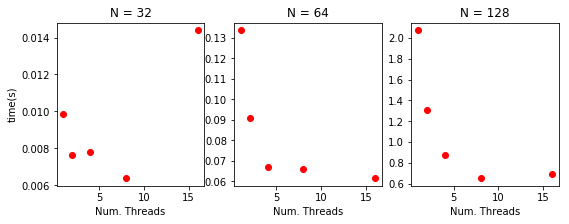
\includegraphics[width=100mm]{scaling.png}
	\caption{Scaling}
	\label{fig:scaling}
\end{figure}
\FloatBarrier

For all three problem sizes, the time to finish decreases initially. Ideally it would keep decreasing, but the communication overhead will eventually take over if we apply a large number of threads. When the problem size is small, it takes much longer to finish if we apply many threads. For the other two problem sizes, they seem to reach their speedup plateau.  

%%%% End document
\end{document}
